\documentclass[a4paper,12pt]{article}
\usepackage[utf8]{inputenc}
\usepackage{polski}
\author{Marcin Fabrykowski}
\title{Eksploracja danych\\Projekt}
\usepackage{listings}
\usepackage{graphicx}
\usepackage{verbatim}
\begin{document}
\maketitle
\newpage
\tableofcontents
\newpage
\section{Opis problemu}
Celem projektu jest opracowanie klasyfikatora drzewiastego do klasyfikacji wina na podstawie jego parametrów.\\
Jako zbiór do nauki, został wykorzystany zbiór\\
http://archive.ics.uci.edu/ml/datasets/Wine+Quality
\section{Opis etapu przygotowania danych}
Dane źródłowe zamieszczone na stronie internetowej były zapisane w formacie CVS (załączony plik winequality-white.csv\_orig).\\
Plik wejściowy musiał zostać przekonwertowany na format możliwy do wczytania przez bibliotekę Orange.\\
Należało zastąpić separator ';' tabulatorem separującym, oraz usunąć cudzysłowia z z nagłówkowego wiersza.\\
Efekt konwersji jest widoczny w pliku: winequality-white.csv
\section{Klasyfikator}
Klasyfikator jest operatorem potrafiącym, po wcześniejszym 'nauczeniu', przewidzieć klasyfikowaną wartość na podstawie badanych atrybutów. W naszym przypadku wartością klasyfikowaną jest jakość wina.\\
Podczas tworzenia klasyfikatora, mamy możliwość określenia maksymalnej głębokości drzewa (max\_depth) oraz ilości iteracji przycinania drzewa (m\_pruning).
\section{Wykorzystywane technologie}
Projekt został napisany w języku Python.\\
Do działania, wymagane są następujące biblioteki:
\begin{itemize}
\item SciPy
\item Orange
\item pygraphviz
\end{itemize}
Orange jest biblioteką wspomagającą operacje związane z eksploracją danych. Udostępnia ona narzędzie do przeprowadzania klasyfikacji, regresji, asocjacji oraz kategoryzacji. Orange pozwala na wyeksportowanie danych o drzewach w formacie .dot, które mogą zostać sparsowane przez program graphviz.
Pygraphviz jest bindingiem do graphviza i pozwala na generowanie diagramów z plików .dot.
\section{Dobór parametrów}
W celu dobrania optymalnego zestawu parametrów, przeprowadzone zostały testy na procent poprawnie rozpoznanych elementów.\\
Badanymi atrybutami są: wysokość drzewa oraz puring.\\
Poniżej zamieszczam wyniki przeprowadzonych testów.\\
%wYNIKI
\begin{verbatim}
{'m_pruning': 0, 'max_depth': 10} CA: 0.4479
{'m_pruning': 0, 'max_depth': 50} CA: 0.4563
{'m_pruning': 0, 'max_depth': 100} CA: 0.4879
{'m_pruning': 0, 'max_depth': 200} CA: 0.5619
{'m_pruning': 0, 'max_depth': 300} CA: 0.6066
{'m_pruning': 0, 'max_depth': 400} CA: 0.6088
{'m_pruning': 0, 'max_depth': 500} CA: 0.6088
{'m_pruning': 0, 'max_depth': 1000} CA: 0.6088
{'m_pruning': 1, 'max_depth': 10} CA: 0.4479
{'m_pruning': 1, 'max_depth': 50} CA: 0.4561
{'m_pruning': 1, 'max_depth': 100} CA: 0.4877
{'m_pruning': 1, 'max_depth': 200} CA: 0.5616
{'m_pruning': 1, 'max_depth': 300} CA: 0.6064
{'m_pruning': 1, 'max_depth': 400} CA: 0.6086
{'m_pruning': 1, 'max_depth': 500} CA: 0.6086
{'m_pruning': 1, 'max_depth': 1000} CA: 0.6086
{'m_pruning': 10, 'max_depth': 10} CA: 0.4477
{'m_pruning': 10, 'max_depth': 50} CA: 0.4508
{'m_pruning': 10, 'max_depth': 100} CA: 0.4824
{'m_pruning': 10, 'max_depth': 200} CA: 0.5412
{'m_pruning': 10, 'max_depth': 300} CA: 0.5772
{'m_pruning': 10, 'max_depth': 400} CA: 0.5776
\end{verbatim}
Na tej podstawie został wybrany zestaw: \{m\_pruning: 10, max\_depth: 300\} ponieważ nie widać zwiększenia skuteczności przy dalszym zwiększaniu wysokości drzewa.\\
Ponadto, wybrano wartość m\_pruning na poziomie 10, ponieważ powoduje nieznaczny spadek skuteczności, przy znacznym zmniejszeniu ilości elementów.
W przypadku pruningu na poziomie 0 - 3441 elementów drzewa, oraz pruning równy 10 - 2519 elementów.
\section{Działanie programu}
Na początku następuje sprawdzenie czy w systemie znajdują się wymagane moduły oraz załadowanie ich.\\
Następnie następuje wczytanie danych wejściowych z pliku csv do tabeli systemu Orange.\\
Po wczytaniu danych, następuje wygenerowanie klasyfikatora dla wczytanych danych oraz ustawionych parametrów tego klasyfikatora.\\
Mając wygenerowanie drzewo klasyfikujące, zapisujemy je do pliku w formacie .dot.\\
Wygenerowany plik .dot zostaje przetworzony przez moduł pygraphviz w celu wygenerowanie pliku graficznego PNG przedstawiającego otrzymamy klasyfikator.
\section{Prezentacja wyników}
Wynikiem działania programu jest klasyfikator drzewiasty przedstawiony na rysunku załączonym do projektu.
%\begin{figure}
%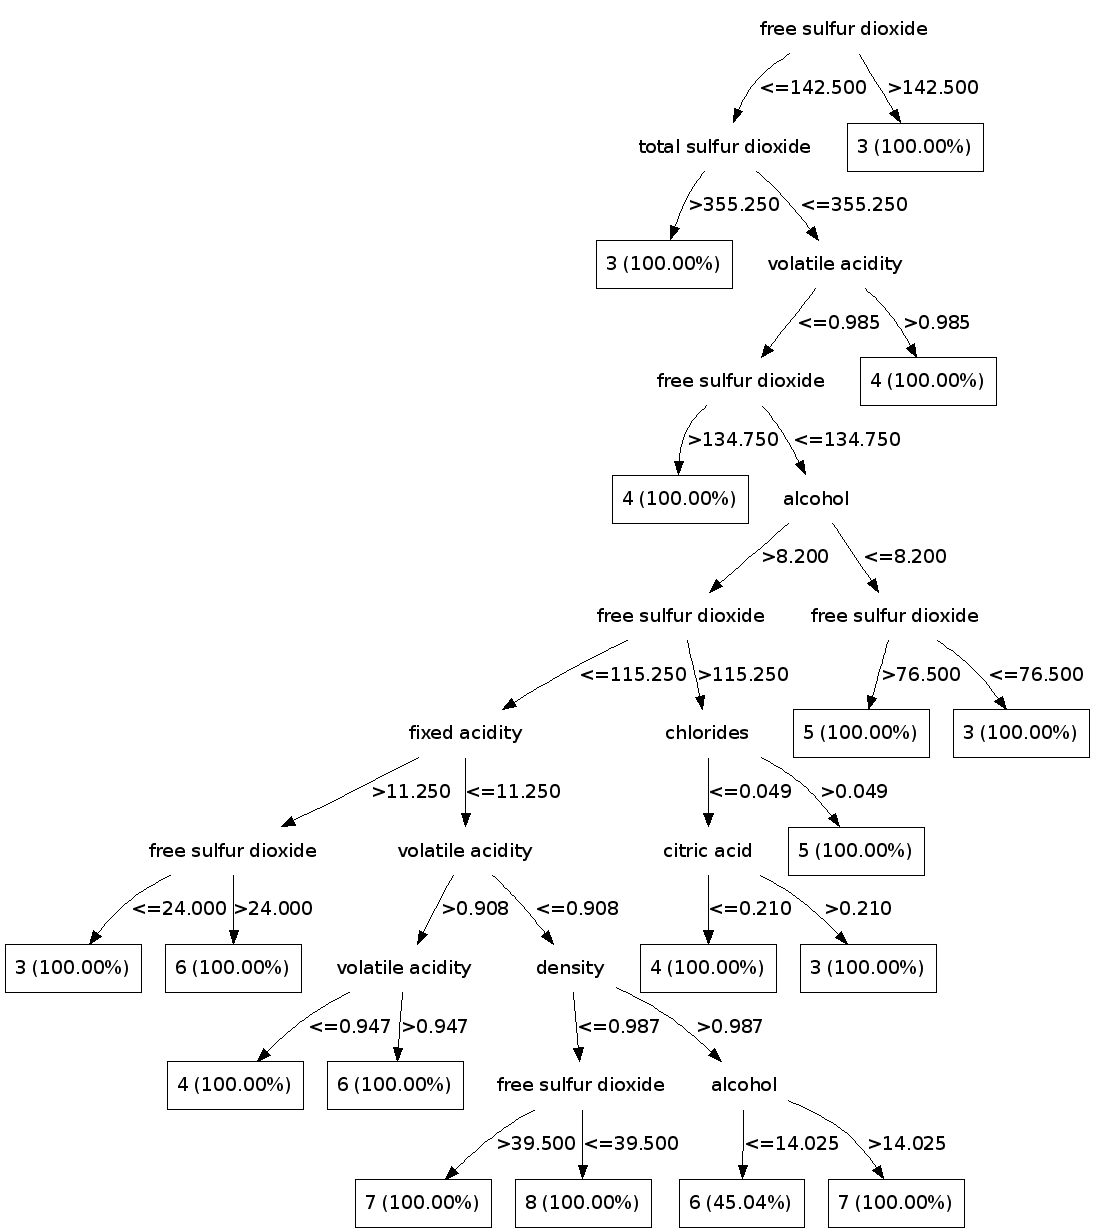
\includegraphics[width=15cm]{FabrykowskiMarcin.png}
%\caption{Reprezentacja graficzna klasyfikatora}
%\label{fig:klasyfikator}
%\end{figure}
\section{Wnioski}
Zauważamy, że użyty klasyfikator nie daje nam 100\% skuteczności rozpoznania i przewidywania wyników, jednak mimo to, uważasz wykorzystywanie technik eksploracji danych za zasadne, ponieważ bez nic nie mielibyśmy żadnych informacji o możliwym zachowaniu jednostek.\\
Nie otrzymujemy odpowiedzi "co się stanie", ale jedynie "co może się stać", a to w technikach marketingowych jest często bardzo dużo.
\end{document}
